\section{NP-complete problems involving sets and numbers.}

\subsection{Disposition}

\begin{enumerate}
 \item \textbf{Theorem 9.9:} \textit{3SAT $\leq$ TRIPARTITE MATCHING}
    \subitem Bevis
 \item \textbf{Collary:} \textit{EXACT COVER BY 3-SETS, SET COVERING and SET PACKING are NPC}
    \subitem Vis for EXACT COVER BY 3-SETS
 \item \textbf{Theorem:} \textit{EXACT COVER BY 3-SETS $\leq$ KNAPSACK}
    \subitem Bevis
\end{enumerate}

\subsection{Emne detaljer}

Følgende afsnit indeholder detaljer om hvert punkt i dispositionen ovenfor (og
muligvis flere ting også).

\subsubsection{Def. P, NP, NP-hard \& NPC}

Lad os starte med lige at kigge på de kompleksitetsklasser vi har arbejdet med
her i kurset.
\begin{center}
 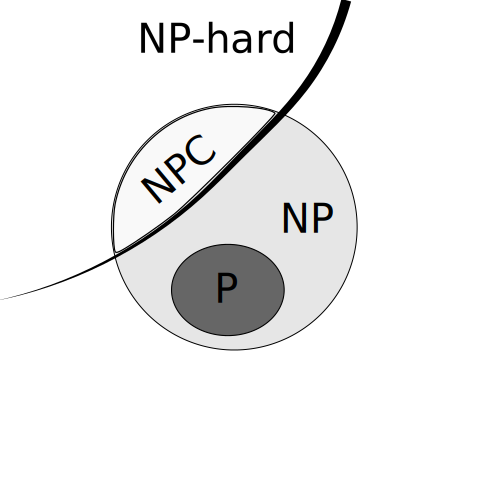
\includegraphics[bb=0 0 400 400,scale=0.3]{img/PNPNPC.png}
 % PNPNPC.png: 1667x1667 pixel, 300dpi, 14.11x14.11 cm, bb=0 0 400 400
\end{center}

\subsubsection{Theorem 9.9 - 3SAT $\leq$ TRIPARTITE MATCHING }

\textbf{TODO: } Følgende bevis har jeg ikke ordentligt forstået og kan meget
vel være forkert hernede.. Tjek den efter meget grundigt og få ekstra kilder
hvorfra du kan verificere nedenstående.. Beviset fuldføres heller ikke helt,
som kan ses nedenfor. \\
~\\
Nu hvor vi har fastlagt at 3SAT er i NPC, så kan vi bruge den til at reducere
videre. Så det første vi vil kigge på er et beslutningsproblem relateret til
set, kaldet TRIPARTITE MATCHING (oversat: treparts matching)

TRIPARTITE MATCHING problemet er følgende: Vi er givet tre sæt $B$, $G$ og $H$
respektivt indeholdende drenge, piger og hjem. Hvor hver af disse sæt
indeholder $n$ elementer og vi har en relation $T \subseteq B \times G \times
H$. Findes der nu et sæt af $n$ tripler i $T$, hvor ingen to af disse har
komponenter til fælles. \\

Altså sagt på en anden måde, kan vi finde $n$ tripler hvor hver dreng er koblet
med en pige og disse så er placeret i et hjem.

Dette problem er NP-Complete, hvilket vi så nu vil vise.
\\
~\\
\textbf{Theorem 9.9:} TRIPARTITE MATCHING $\in$ NPC

\begin{proof}
 Vi vil vise at TRIPARTITE MATCHING er i NPC ved at reducerer fra 3SAT. Vi har
 altså en CNF formel $f$ i 3SAT med variabler $x_1,\hdots,x_n$ og skal så nu
 konstruere instanser af TRIPARTITE MATCHING på baggrund af dette vha. en
 polynomieltids reduktion $r$.

 Måden hvorpå vi konstruerer disse instanser er vha. en såkaldt
 ``choice-consistency'' gadget, som illustreret nedenfor.
 \begin{center}
 
\includegraphics[bb=0 0 479 422,scale=0.5]{img/choiceConsistency.png}
 % choiceConsistency.png: 1997x1760 pixel, 300dpi, 16.91x14.90 cm, bb=0 0 479 422
\end{center}
Konstruktionen følger så denne opskrift:
\begin{enumerate}
 \item For hver variabel $x_i$ i $f$, konstruer en ``choice-consistency'' gadget
    \subitem (a) Lad $k$ være antallet af forekomster af $x_i$, eller $\neg x_i$, i $f$ (den af dem hvor der er flest).
    \subitem (b) Konstruer vores gadget med $k$ drenge, $k$ piger og $2k$ hjem. Hvor drenge og piger placeres efter hinanden i en slags ``ring'' hvor hjemene er placeret ud for dem i en trekant repræsenterende tripler.
    \subitem (c) Hjemene $h_{2i-1}$ repræsenterer forekomster af $x$, hvor $h_{2i}$ repræsenterer forekomster af $\neg x$, for $i = 1,\hdots,k$. (hvis antallet af forekomster af de to er ulige, så vil nogle $h_i$'er blot være utildelt)
    \subitem (d) De $k$ drenge og $k$ piger indgår ikke i tripler af $T$ udover dem der er vist i figuren. Så hvis en matching eksisterer, så er $b_i$ matched med $g_i$ og $h_{2i}$ eller med $g_{i-1}$ ($g_k$ hvis $i=1$) og $h_{2i-1}$, for $i = 1,\hdots,k$. Hvis den første var tilfældet, så er $T(x)=true$ og hvis det er den anden så er $T(x)=false$. \\
    Dette betyder, at en given variabel $x$ altid vælger en tildeling og alle forekomster af variablen har konsistente værdier.
 \item For hver klausul i $f$, konstruer en triple med en dreng $b$ og en pige
	 $g$. De eneste tripler $b$ og $g$ indgår i, er så tripler på formen
	 $(b,g,h)$ hvor $h$ er de 3 hjem svarende til de 3 forekomster af literals
	 i den pågældende klausul. Ideen er så, at hvis en af disse 3 hjem blev
	 efterladt ubeboet når variabler blev tildelt værdier, så betyder det at
	 huset svarer til en ``true'' literal og klausulen er derfor
	 tilfredsstillet. Hvis alle 3 literals i klausulen er ``false'', så kan $b$
	 og $g$ ikke tildeles et hjem. \\
 Illustreret nedenfor:
\end{enumerate}
\begin{center}
 \includegraphics[bb=0 0 292 174]{img/choiceConsistencySub.png}
 % choiceConsistencySub.png: 389x232 pixel, 96dpi, 10.29x6.14 cm, bb=0 0 292 174
\end{center}


Hermed er konstruktionen færdig, dog med den detalje at der pt. er flere hjem
end drenge og piger i konstruktionen. Hvis der er $m$ klausuler, så er der $3m$
forekomster hvorfor der mindst er $H=3m$ hjem (for hver variabel har vi mindst
lige så mange hjem som forekomster). På den anden side har vi $\frac{H}{2}$
drenge i vores gadgets og yderligere $m \leq \frac{H}{3}$ i vores klausul
constraint del.

Lad os antage at mængden af huse vi har for meget er $l$, så kan vi introducere
$l$ flere drenge og $l$ flere piger, således $|B| = |G| = |H|$. For hver af
disse $l$ drenge og piger tilføjes så $|H|$ tripler der forbinder til alle
hjem. Disse sidste $l$ drenge og piger kan så ses som ``easy to please'' par,
da de blot bruges til at udfylde hvad end hjem der er ubeboet.\\
~\\
Vi påstår så nu, at en tripartite matching eksisterer hvis og kun hvis den
oprindelige boolske formel var tilfredsstillet. Dette kan vi se ved 
 
\end{proof}

\subsubsection{Collary: Andre problemer med sæt i NPC}

Nu hvor vi har bevist at TRIPARTITE MATCHING er NP-Complete, så bringer det
nærmest automatisk en række andre problemer ind i den kategori, da visse andre
problemer med sæt blot er forskellige afarter heraf. Her kigger vi specifikt på
3 hurtigt, nemlig EXACT COVER BY 3-SETS, SET COVERING og SET PACKING.
Problemerne er defineret således:

\begin{description}
 \item[SET COVERING:] Vi er givet en familie $F = \left\lbrace S_1,\hdots,S_n
	 \right\rbrace$ af subsets af et endeligt sæt $U$ og et budget $B$. Er der
	 et sæt af $B$ sæt i $F$ hvor deres foreningsmængde er $U$?
 \item[SET PACKING:] Vi er givet en familie $F = \left\lbrace S_1,\hdots,S_n
	 \right\rbrace$ af subsets af et sæt $U$ og et mål $K$. Er der $K$ parvis
	 disjunkte sæt i familien $F$?
 \item[EXACT COVER BY 3-SETS:] Vi er givet en familie $F = \left\lbrace
	 S_1,\hdots,S_n \right\rbrace$ af subsets af et sæt $U$, således at
	 $|U|=3m$ for en given int $m$ og $|S_i|=3$ for alle $i$. Er der $m$ sæt i
	 $F$ som er disjunkte og har $U$ som deres foreningsmængde?
\end{description}

Alle disse problemer kan vises at være NP-Complete, da de alle er
generaliseringer af TRIPARTITE MATCHING.\\
~\\
\textbf{Collary:} EXACT COVER BY 3-SETS, SET COVERING og SET PACKING $\in$ NPC

\begin{proof}
Vi starter med at reducere TRIPARTITE MATCHING til EXACT COVER BY 3-SETS, for
derved at vise, at sidstnævnte er i NPC.

Givet sæt $B$, $G$ og $H$, samt relationen $T \subseteq B \times G \times H$ i
TRIPARTITE MATCHING, så vil vi konstruere disse dele i EXACT COVER BY 3-SETS
vha. en polynomiel reduktion $r$. Således kan vi sige, at EXACT COVER BY
3-SETS har $m$ sæt der er disjunkte og har foreningsmængde $U$, hvis og kun
hvis TRIPARTITE MATCHING har en fyldestgørende matching.

Måden vi gør det på er ved at dele $U$ i sidstnævnte op, således $U = B
\bigcup G \bigcup H$ hvor disse $B$, $G$ og $H$ selvfølgelig er disjunkte. Til
enhver triple $t_i=(b,g,h) \in T$ associerer vi så et sæt $S_i=\left\lbrace
b,g,h \right\rbrace$ Således får vi, at foreningsmængden af de $m$ sæt kun er
$U$ såfremt $T$ er en fyldestgørende matching, og vice-versa.

Altså har vi at EXACT COVER BY 3-SETS $\in$ NPC.\\
~\\
Et endnu nemmere bevis kan føres for SET COVERING ved at reducere fra EXACT
COVER BY 3-SETS. Vi lader blot $F$ udelukkende bestå af sæts med 3 elementer,
lader $U$ bestå af $3m$ elementer og sætter budgettet $B=m$, derved får vi
EXACT COVER BY 3-SETS direkte. 

Så SET COVERING $\in$ NPC.\\
~\\
Det tilsvarende kan gøres igen for en reducering fra EXACT COVER BY 3-SETS til
SET PACKING, hvor $F$ og $U$ sættes som før, og målet $K=m$. 

Således får vi også her at SET PACKING $\in$ NPC.
\end{proof}

\subsubsection{Theorem: (EXACT COVER BY 3-SETS $\leq$ KNAPSACK)}

Nu hvor vi har vist at EXACT COVER BY 3-SETS er NP-Complete, så kan vi nu bruge
den viden til at lave endnu en reduktion. Vi vil kigge på problemet kaldet
KNAPSACK.

Problemet går ud på at vi må vælge nogle genstande blandt $n$ samlede
genstande. Genstand $i$ har værdi $v_i$ og vægt $w_i$, hvor begge er positive
heltal. Der er desuden en max vægt på $W$, som er den maksimale vægt vores
genstande tilsammen må veje. Vi skal så nu vælge genstande, uden gentagelser,
således vi maksimerer den totale værdi med den constraint at den samlede vægt
ikke må overstige $W$.

Vi leder altså efter et subset $S \subseteq \left\lbrace 1,\hdots,n
\right\rbrace$ således at $\sum_{i \in S} w_i \leq W$ og $\sum_{i \in S} v_i$
er så stor som mulig.

I beslutningsproblem varianten har vi desuden et mål $K$ og vi ønsker at finde
et subset $S \subseteq \left\lbrace 1, \hdots, n \right\rbrace$ således
$\sum_{i \in S} w_i \leq W$ og $\sum_{i \in S} v_i \geq K$.

Vi vil så nu bevise at KNAPSACK $\in$ NPC ved at bevise et relateret problem.\\
~\\
\textbf{Theorem 9.10:} KNAPSACK $\in$ NPC

\begin{proof}
 I dette bevis vil vi reducere fra EXACT COVER BY 3-SETS, men vi vil ikke
 reducere til KNAPSACK. I stedet vil vi begrænse problemet og fokusere på et
 special case, som vi så vil bevise er NPC. Dette special case kalder vi SUBSET
 SUM og det eneste vi ændrer imellem de to, er at $K=W$ og for hver genstand
 $i$ sætter vi $v_i = w_i$.

Altså har vi nu et problem hvor vi er givet et sæt af $n$ heltal
$v_1,\hdots,v_n$ og endnu et heltal $K$. Vi ønsker nu at finde ud af om et
givet subset summer præcist op til $K$.\\

 Vi har altså en instance af EXACT COVER BY 3-SETS med sæt $\left\lbrace S_1,
 S_2,\hdots,S_n \right\rbrace$, hvor vi spørger om der er disjunkte sæt hvor
 deres foreningsmængde er sættet $U = \left\lbrace 1, 2, \hdots, 3m
 \right\rbrace$. Vi tænker på disse sæt som bit vektorer i $\left\lbrace 0,1
 \right\rbrace^{3m}$, således de også kan tænkes som binære heltal og forening
 mellem disse sæt nu ligner heltalsaddition til forveksling (eksempel ses
 nedenfor)
\begin{center}
 
\includegraphics[bb=0 0 389 186,scale=0.5]{img/KNAPSACK.png}
 % KNAPSACK.png: 1620x773 pixel, 300dpi, 13.72x6.54 cm, bb=0 0 389 186
\end{center}
Vores mål er nu at finde et subset af disse binære heltal der summerer op til
$K=2^n -1$, altså en bitstreng med rene 1-taller, svarende til hele $U$.
Reduktionen er nu fuldendt, men der er en mindre additionsbug. 

Problemet er, at binær heltalsaddition ikke er det samme som mængdeforening, da
binær heltalsaddition har såkaldt ``carry'' (i.e. $1 + 1 \rightarrow 0, carry
1$, så $1 + 1 = 0 + 1 \times 10$ hvilket giver $10$ i binær). F.eks. er
$3+5+7=15$ i bitvektorform $0011 + 0101 + 0111 = 1111$, men i de tilsvarende
sæt er det $\left\lbrace 3,4 \right\rbrace, \left\lbrace 2,4 \right\rbrace$ og
$\left\lbrace 2,3,4 \right\rbrace$, som er ikke disjunkte (som de burde) og
deres foreningsmængde heller ikke $\left\lbrace 1,2,3,4 \right\rbrace$.

Der er dog en simpel og smart måde at undgå dette problem på. I stedet for at
have disse vektorer af heltal i base 2, så hav dem i base $n+1$. På den måde
bliver sæt $S_i$ til heltal $v_i = \sum_{j \in S_i} (n+1)^{3m-j}$.

Siden der nu ikke er noget ``carry'' i additionen af op til $n$ af disse numre,
så er det nu klart at se, at disse heltal summer op til $K = \sum_{j=0}^{3m-1}
(n+1)^j$ hvis og kun hvis der er et exact cover iblandt $\left\lbrace S_1, S_2,
\hdots, S_n \right\rbrace$.

Vi har altså at EXACT COVER BY 3-SETS $\leq$ SUBSET SUM og derved at SUBSET SUM
$\in$ NPC, hvilket også vil sige KNAPSACK $\in$ NPC. 
\end{proof}
